    \def\cmsBoxWidth{43cm}
    \def\firstRowHeight{31cm}
    \node[boxStyle, text width=\cmsBoxWidth, anchor=north west, minimum height=\firstRowHeight] (cmsBox) at (-40, 41){
       \begin{minipage}{\cmsBoxWidth}
          {\small
          The \textbf{Compact Muon Solenoid (CMS) experiment} is a particle-physics experiment at the \textbf{Large Hadron Collider} (LHC), the world's most powerful particle accelerator located at CERN, Geneva.
          CMS is designed to detect a wide range of particles and phenomena produced in the LHC's high-energy proton-proton collisions. During its first years of operation, CMS achieved many new precision results on
          the Standard Model and limits on new physics beyond the Standard Model, as well as the long awaited discovery of the Higgs boson.
          In the previous years (2015-2018), CMS took data at an \textbf{unprecedented centre-of-mass energy of 13 TeV}, and at a rate of 40 million collisions per second.
          In your master thesis, you will use these data for precision measurements or searches for new physics, acquiring useful knowledge of data analysis
          techniques for your future academic or professional career!
          \vspace{5mm}
          \begin{figure}
            \centering
             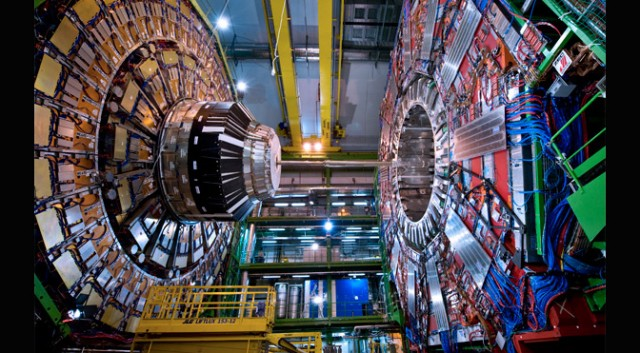
\includegraphics[height=12cm,trim=50 0 50 0,clip]{{general/CMS}.jpg}      
             \hspace{2cm}
             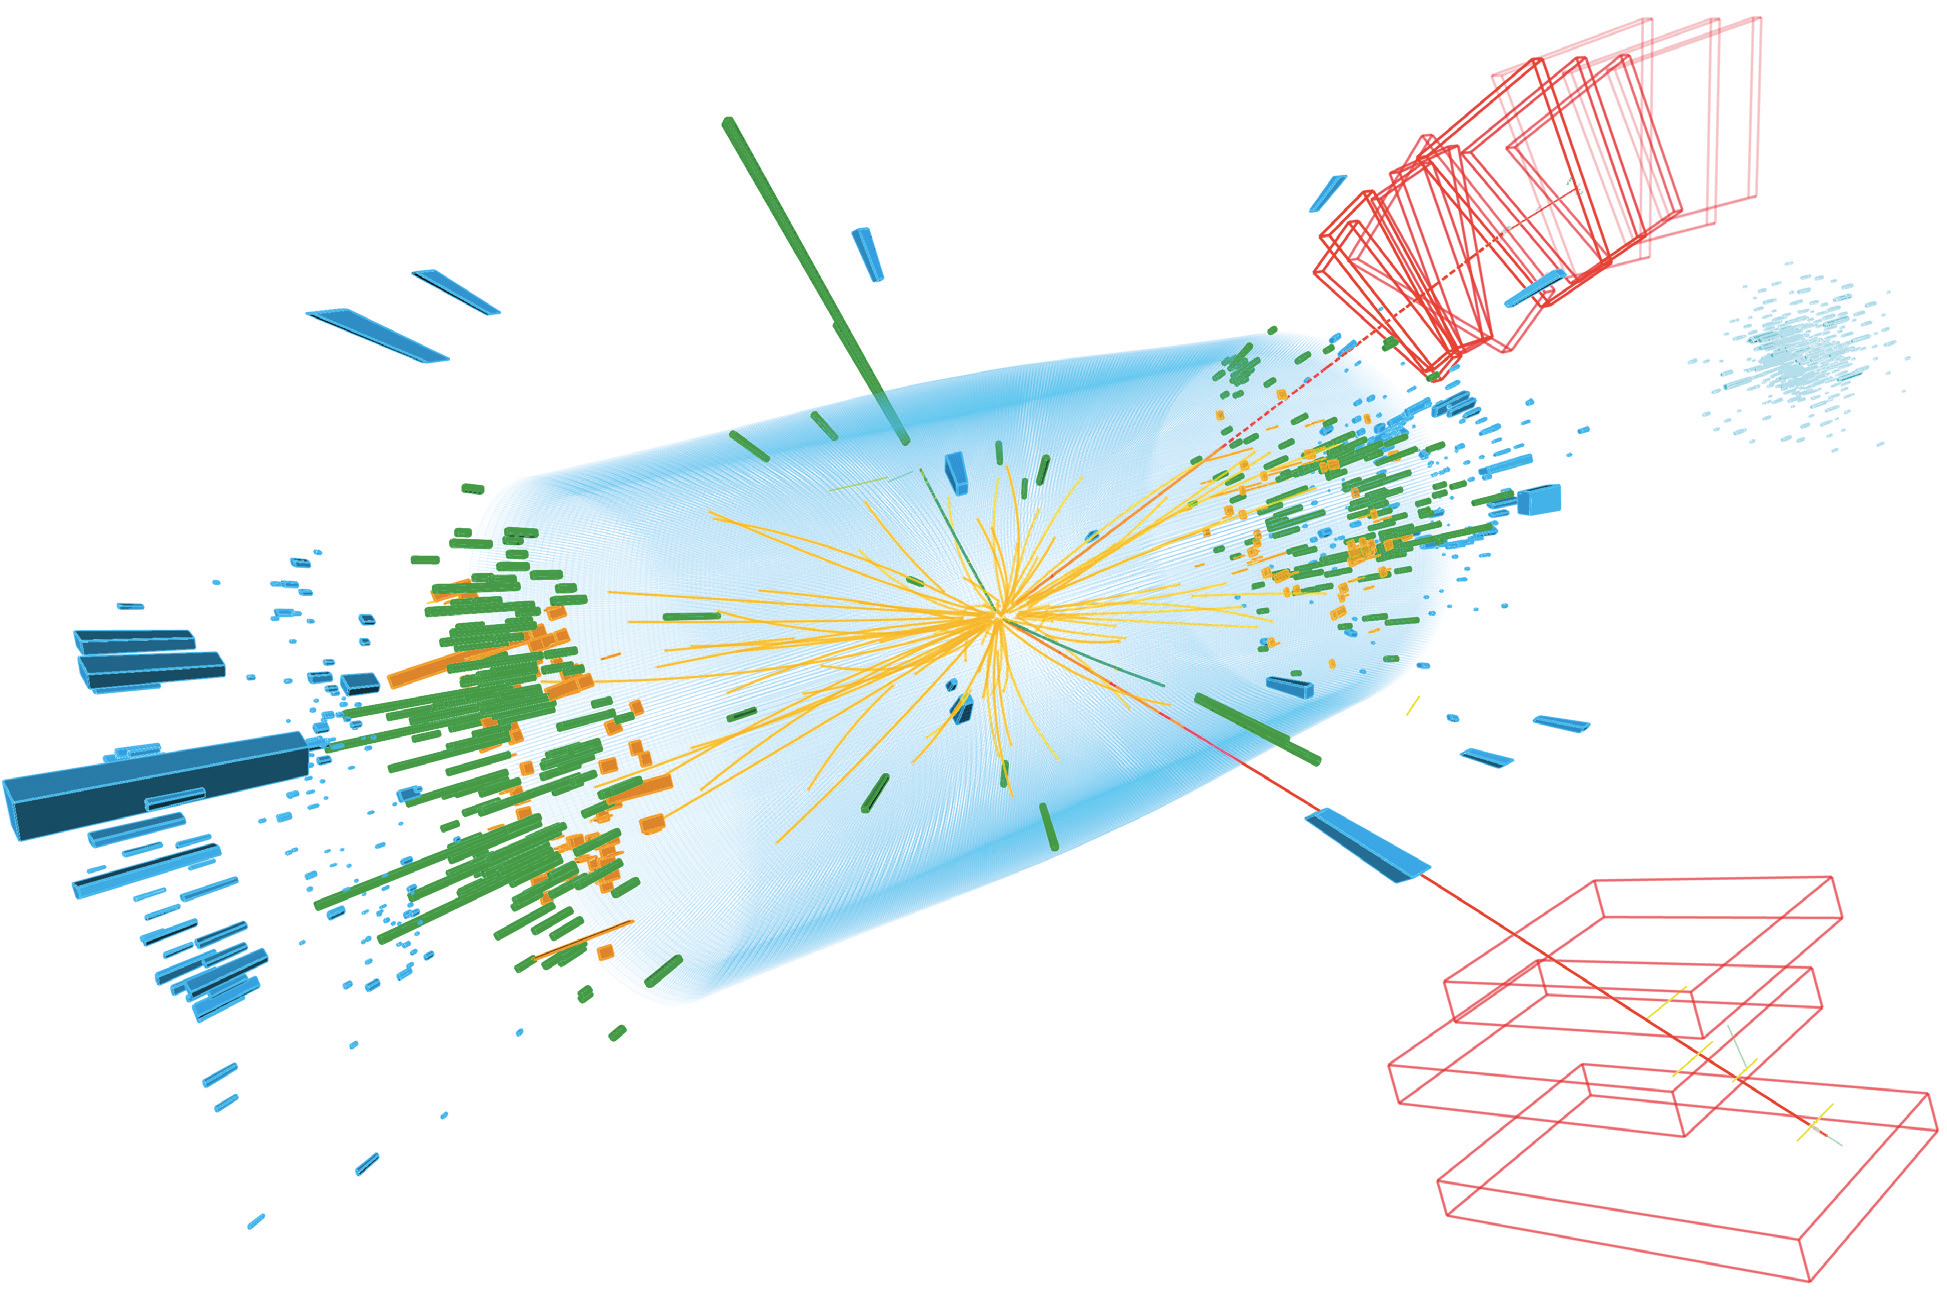
\includegraphics[height=12cm]{{general/eventDisplay}.png}   
          \end{figure}
          \vspace{5mm}
          \color{white} The CMS experiment is one of the largest international scientific collaborations in history, involving 4300 particle physicists, engineers, technicians, students and support staff from 229 universities and institutes in 51 countries.
       }\end{minipage}
   };
   \node[green] at ($(cmsBox.south east)+(-14,18.3)$){$e$};
   \node[green] at ($(cmsBox.south east)+(-7.2,11.7)$){$e$};
   \node[red] at ($(cmsBox.south east)+(-4,8)$){$\mu$};
   \node[red] at ($(cmsBox.south east)+(-4,18)$){$\mu$};


 %   \node[fancytitle, left=\titleOffset] at (cmsBox.north east) {The CMS detector at the LHC};

